\section{Modello di Ising 1D}

Il modello di Ising 1D è uno dei pochi modelli della meccanica statistica che presenta una soluzione esatta.
Il reticolo che prendiamo in considerazione in questo caso è lineare, tale per cui ogni sito reticolare presenta 
solo due primi vicini. Lavorando con condizioni periodiche al contorno, l'N-esimo spin diventa un vicino del 
primo ed il sistema si chiude ad anello, come è possibile apprezzare in Figura \ref{fig: Ising1D_pbc}.

\begin{figure}[h!]
    \centering
    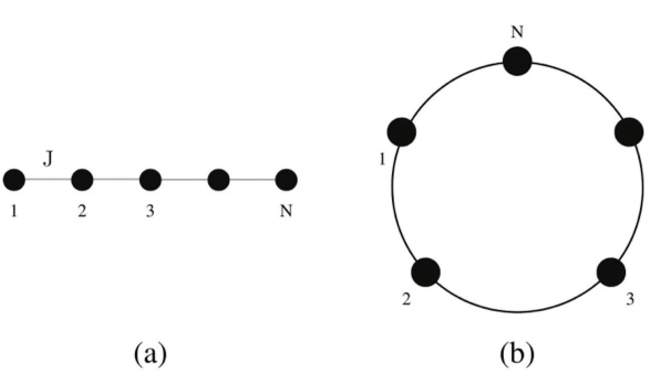
\includegraphics[width=0.7\textwidth]{Immagini/Ising1D_pbc.png}
    \caption{L'immagine (a) è un esempio di modello di Ising 1D senza pbc, mentre in (b) si può apprezzare 
    come la catena si chiuda su se stessa nel caso di condizioni periodiche al contorno. }
    \label{fig: Ising1D_pbc}
\end{figure}

Sebbene il modello di Ising 1D ammetta soluzione esatta, è istruttivo lavorare inizialmente con una teoria di campo 
medio, in cui il termine d'interazione presente nell'Hamiltoniana viene sostituito da un termine efficace (di campo 
medio appunto), andando a trascurare le fluttuazioni degli spin.





\subsection{Teoria di campo medio}

Il punto di partenza di una teoria di campo medio è la semplificazione del temine d'interazione presente nell'Hamiltoniana. Nel  
caso del modello di Ising mono-dimensionale l'interazione fra spin primi vicini può essere riscritta come

\begin{equation}
    \sigma_i \sigma_j\,=\,\left(\sigma_i\,-\,m\,+\,m\right)\left(\sigma_j\,-\,m\,+\,m\right)\,=\,-m^2\,+\,m\sigma_i\,+\,m\sigma_j\,+\,\left(\sigma_i\,-\,m\right)\left(\sigma_j\,-\,m\right),
    \label{eq: int_mf}
\end{equation}

dove l'ultimo termine della somma misura le fluttuazioni fra spin. L'approssimazione di campo medio consiste nel trascurare 
completamente l'ultimo termine, in modo tale che tutti gli spin risultino essere disaccoppiati fra loro e risulti più immediato il 
calcolo della funzione di partizione. L'Hamiltoniana di campo medio risulta quindi 

\begin{equation}
    H_{MF}\,=\,-\frac{J}{2} \sum_{\left<i,j\right>} \left[-m^2\,+\,m\left(\sigma_i\,+\,\sigma_j\right)\right]\,-\,h\sum_{i}\sigma_i,
    \label{eq: ham_mf}
\end{equation}

da cui è immediato il calcolo della funzione di partizione 

\begin{equation}
    Q_{MF}\,=\,\sum_{\left\{\sigma\right\}} e^{-\beta H_{MF}}\,=\,\exp{\left(-\frac{\beta J m^2 N n_{nn}}{2}\right)} \left\{2 \cosh{\left[\beta \left(J n_{nn} m\,+\,h\right)\right]}\right\}^N.
    \label{eq: part_MF_Ising1D}
\end{equation}

Nella relazione precedente la quantità $n_{nn}$ è il numero il numero di coordinazione del reticolo, ossia il numero di primi vicini per la 
geometria presa in considerazione. L'energia libera per particella è data da 

\begin{equation}
    \frac{F}{N}\,=\,-\frac{k_B T}{N} \ln{\left(Q_{MF}\right)}\,=\,\frac{JM^2n_{nn}}{2}\,-\,\frac{1}{\beta}\ln{\left\{2 \cosh{\left[\beta\left(h\,+\,Jn_{nn}m\right)\right]}\right\}}
    \label{eq: freeE_MF_Ising1D}
\end{equation}




\subsection{Soluzione esatta}

Considerare un sistema con condizioni periodiche al contorno, come (b) in Figura \ref{fig: Ising1D_pbc}, consente 
di scrivere l'Hamiltoniana in forma simmetrica come 

\begin{equation}
    H\,=\,-J\sum_{i} \sigma_i \sigma_{i+1}\,-\,\frac{h}{2}\sum_{i} \left(\sigma_i\,+\,\sigma_{i+1}\right),
    \label{eq: ising_ham_sim}
\end{equation}

dato che $\sigma_{N+1}\,=\,\sigma_1$. La funzione di partizione del sistema è data dalla somma su tutte le possibili 
configurazioni del sistema, che si traduce in 

\begin{equation}
    Q\left(h,\,T\right)\,=\,\sum_{\sigma_1=\pm 1} \cdots \sum_{\sigma_N=\pm 1} \exp{\left\{\beta\left[J\sum_i \sigma_i \sigma_{i+1}\,+\,\frac{h}{2}\sum_i \left(\sigma_i\,+\,\sigma_{i+1}\right)\right]\right\}}
    \label{eq: part_func}
\end{equation}

Definendo una matrice P come

\begin{equation}
    P = \begin{pmatrix}
    e^{\beta\left(J\,+\,h\right)} & e^{-\beta J} \\\\
    e^{-\beta J} & e^{\beta\left(J\,-\,h\right)}
    \end{pmatrix}
    \label{eq: mat_P}
\end{equation}

è possibile riscrivere la funzione di partizione in termini matriciali

\begin{equation}
    Q\left(h,\,T\right)\,=\,\sum_{\sigma_1=\pm 1} \cdots \sum_{\sigma_N=\pm 1} \langle \sigma_1 | P | \sigma_2 \rangle \langle \sigma_2 | P | \sigma_3 \rangle \cdots \langle \sigma_{N-1} | P | \sigma_N \rangle \langle \sigma_N | P | \sigma_1 \rangle 
    \label{eq: part_func_mat}
\end{equation}

Notando che sono presenti $N\,-\,1$ completezze, è possibile procedere ad una semplificazione estrema della relazione 
\eqref{eq: part_func_mat} che consente di apprezzare come la funzione di partizione altro non sia che la traccia della matrice P 
elevata alla N. 

\begin{equation}
    Q\left(h,\,T\right)\,=\,\sum_{\sigma_1=\pm 1} \langle \sigma_1 | P^N | \sigma_1 \rangle \,=\,Tr\left(P^N\right)\,=\,\lambda_1^N\,+\,\lambda_2^N,
    \label{eq: part_func_simp}
\end{equation}

dove $\lambda_1$ e $\lambda_2$ sono gli autovalori della matrice P. La loro determinazione richiede la soluzione di un problema agli 
autovalori, che porta a 

\begin{equation}
    \lambda_{1,2}\,=\,e^{\beta J} \cosh{\left(\beta h\right)}\,\pm\,\sqrt{e^{- 2 \beta J}\,+\,e^{2 \beta J} \sinh^2{\left(\beta h\right)}}.
    \label{eq: autoval_P}
\end{equation}

Una ottima approssimazione, quando il numero di spin preso in considerazione è elevato, consiste nel trascurare il secondo autovalore 
dato che 

\begin{equation}
    \lim_{N \to \infty} \left(\frac{\lambda_2}{\lambda_1}\right)^N\,=\,0.
    \label{eq: approx_Q}
\end{equation}

L'energia libera di Helmholtz, dalla quale è possibile determinare tutta la termodinamica del sistema, risulta quindi

\begin{equation}
    A\left(h,\,T\right)\,=\,-k_B T \ln{\left[Q\left(h,\,T\right)\right]}\,\simeq\,-Nk_BT \ln{\left(\lambda_1\right)}.
    \label{eq: en_lib}
\end{equation}



\subsubsection{Magnetizzazione}

Dall'energia libera di Helmholtz è possibile ricavare la magnetizzazione per spin, che costituisce il parametro d'ordine del 
sistema in analisi ed in quanto tale consente di caratterizzare le transizioni di fase. In particolare, tale quantità si 
ottiene come derivata di $A\left(h,\,T\right)$ rispetto al campo magnetico applicato, in modo tale che

\begin{equation}
    m\,=\,-\left(\frac{\partial A/N}{\partial h}\right)_T\,=\,\frac{\sinh{\left(\beta h\right)}}{\sqrt{e^{-4\beta J}\,+\,\sinh^2\left(\beta h\right)}}
    \label{eq: magn_Ising1D_corr}
\end{equation}

Notiamo che quando $h\,\to\,0$ la magnetizzazione tende ad un valore nullo a tutte le temperature finite. Questo evidenzia 
come sia impossibile avere magnetizzazione spontanea, e quindi una transizione di fase, ad ogni temperatura finita T: tale risultato 
è in contrasto con quanto previsto dalla teoria di campo medio, che oltre a fornire gli esponenti critici sbagliati, suggerisce la 
presenza di ordine a $T\,\neq\,0$, che è un risultato non fisico come mostra la soluzione esatta. Quando si ha $T\,=\,0$ $m$ satura ad 
uno per ogni valore del campo magnetico, il che implica perfetto ordine nel sistema; questo significa che la temperatura critica 
$T_c$ coincide con lo zero assoluto. E' anche possibile calcolare la suscettività magnetica, la quale diverge 
quanto $T\,\to\,0$, che è il comportamento che ci si aspetterebbe la punto critico.


\subsubsection{Correlazioni fra spin}

Consideriamo ora un modello di Ising costituito da un reticolo lineare aperto, senza più condizioni al contorno periodiche, 
come quello in Figura \ref{fig: Ising1D_open}. 

\begin{figure}[H]
    \centering
    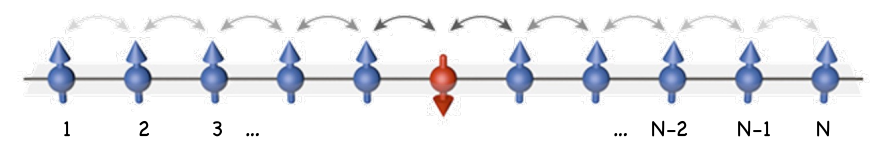
\includegraphics[width=0.7\textwidth]{Immagini/Ising1D_open.png}
    \caption{Esempio di catena di spin per la determinazione della funzione di correlazione fra due spin.}
    \label{fig: Ising1D_open}
\end{figure}

La funzione di correlazione fra due spin $\sigma_i$ e $\sigma_j$ è definita come

\begin{equation}
    G_{ij}\,=\,\left<\sigma_i \sigma_j\right>\,-\,\left<\sigma_i\right>\left<\sigma_j\right>
    \label{eq: def_corr_fun_Ising1D}
\end{equation}

e consente di valutare se due spin sono correlati o meno. Nel caso del modello di Ising 1D la funzione di correlazione 
risulta essere

\begin{equation}
    G_{i, i+r}\,=\,\left(\tanh{\beta J}\right)^r.
    \label{eq: Ising1D_cor}
\end{equation}

Dall'equazione \eqref{eq: Ising1D_cor} è possibile determinare quale sia la lunghezza di correlazione esprimendo la 
$G_{i, i+r}$ come una funzione esponenzialmente decadente della separazione $r$ fra gli spin in analisi. 

\begin{equation}
    G_{i, i+r}\,=\,e^{r\left[\ln{\left(\tanh{\beta J}\right)}\right]}\,=\,e^{-r/\xi},
    \label{eq: Ising1D_corr_exp}
\end{equation}

da cui risulta che la lunghezza di correlazione è pari a 

\begin{equation}
    \xi\,=\,-\frac{1}{\ln{\left[\tanh{\left(J/k_B T\right)}\right]}}.
    \label{eq: lungh_corr}
\end{equation}

Notiamo che la lunghezza di correlazione è sempre maggiore o uguale a zero. Inoltre, quando la temperatura tende a zero, 
$\xi$ diverge ad infinito. Il fatto che questo accada solamente a temperatura nulla evidenzia come non si abbia correlazione 
(e di conseguenza ordine) a lungo raggio fra gli spin per ogni $T\,\neq\,0$.
